\section{Реализация Class-Based WFQ в ядре Linux}

	\subsection{Управление трафиком}

	%Расскать про traffic control (tc) и как он связан с конфигурацией qdisc + Netlink.

	В Linux управление трафиком осуществляется с помощью подсистемы Traffic Control,
	которая предоставляет пользовательский интерфейс с помощью программы \texttt{tc}.
	\texttt{tc} -- это пользовательская программа, которая позволяет настраивать
	дисцплины обслуживания в Linux. Она использует Netlink в качестве
	коммуникационного канала для взаимодействия между пользовательским
	пространством и пространством ядра. Он добавляет новые дисциплины
	обслуживания, классы трафика, фильтры и предоставляет команды для
	управление всеми обозначенными объектами.
	% TCP-IP architecture

	\texttt{tc} предоставляет интерфейс для дисцплины обслуживания,
	представленный структурой \lstinline{struct qdisc_util}, которая
	описывает функции для отправления входящих параметров и печати
	сообщений от ядра. Сообщение, помимо общей информации для подсистемы,
	содержит специфичную для дисциплины структуру с опциями, описываемую
	в заголовке ядра (pkt\_sched.h). 

	Таком образом, для использования дисциплины обслуживания необходимо
	реализовать интерфейс в системе \texttt{tc}. 

	\subsection{Алгоритм выделения канала} 

	???

	\subsection{Описание устройства подсистемы планировки в ядре Linux}
	% Информация из комментариев к ним.
	% Файлы: linux/net/sched/sch_api.c, linux/include/net/{sch_generic.h,pkt_sched.h}. 

	%[Схема пути пакета]

	%В ядре сетевое устройство описывается структурой \lstinline{struct net_device},
	%которая содержит указатель на ассоциированную с устройством дисциплину обслуживания,
	%описываемая структурой \lstinline{struct Qdisc}.

	%Опишем важные для понимания подсистемы поля \texttt{Qdisc}.
	%\begin{itemize}
	%	\item enqueue
	%\end{itemize} 

	В общем случае, дисциплина обслуживания -- это чёрный ящик, который может
	ставить пакеты в очереди и вынимать их из очереди, когда устройство
	готово к отправке, в порядка и во время, определёнными спрятанным в ящике
	алгоритмом. В ядре Linux дисциплины обслуживания представляются в качестве
	модулей ядра, которые реализуют предоставляемый ядром интерфейс.

	Linux поддерживает классовые и бесклассовые дисцплины обслуживания. Примером
	бесклассовой дисциплины служит pfifo\_fast, классовой -- HTB.

	% lartc

	Классы представляют собой одельные сущности в иерархии основной дисциплины.
	Если структура представляет собой дерево, то в классах-узлах могут содержаться
	фильтры, которые определят пакет в нужный класс-потомок. В классах-листьях
	непосредстенно располагаются очереди, которые управляются внутренней дисциплной
	обслуживания (обычно это FIFO). 

	Каждый интерфейс имеет корневую дисцплину (по умолчанию pfast\_fifo), которой
	назначается идентификатор (handle), который используется для обращения к дисциплине.
	Этот идентификатор состоит из двух частей: мажорной (MAJ) и минорной (MIN); мажорная
	часть определяет родителя, минорная -- непосредственно класс.

	\begin{figure}[ht!]
		\centering
		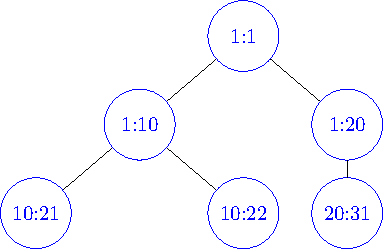
\includegraphics{./pdfimages/class_hierh.pdf}
		\caption{Схема классовой иерархии с использованием идентификаторов MAJ:MIN}
	\end{figure}

	[Возможно, сделать небольшой вывод по описанному и связать его со следующим абзацем.]

	CBWFQ является классовой дисцплиной облуживания, поэтому лучшим вариантом
	её реализации является реализация с использованием механизмов ядра для
	классовых дисциплин.

	\subsection{Описание интерфейса}

	API предосавтляет две функции: \lstinline{register_qdisc(struct Qdisc_ops *ops)}
	и обратную -- \lstinline{unregister_qdisc(struct Qdisc_ops *ops)}, которые регистрируют
	и разрегистрируют дисциплину обслуживания. Важно отметить, что обе эти
	функции принимают в качестве аргумента структуру \lstinline{struct Qdisc_ops},
	которая явным образом идентифицирует дисциплину обслуживания в ядре.

	Структура \texttt{Qdisc\_ops} помимо метаинформации содержит указатели на функции,
	которые должен реализовывать модель дисциплины обслуживания для корректной
	работы в ядре. 

	Следующие функции определяют работу алгоритма.
	\begin{itemize}
		\item \lstinline{enqueue}\\
   		    \lstinline{int enqueue(struct sk_buff *skb, struct Qdisc *sch, struct sk_buff **to_free);} \\
			Фукнкция добавляет пакет в очередь. Если пакет был отброшен, функция
			возращает код ошибки, говорящий о том, был отброшен пришедший пакет или
			иной, чьё место занял новый.
		\item \lstinline{dequeue}\\
			\lstinline{struct sk_buff *dequeue(struct Qdisc * sch);}
			Функция, возвращающая пакет из очереди на отправку. Дисциплина
			может не передавать пакет при вызове этой функции по решению
			алгоритма, в таком случае вернув нулевой указатель; 
			однако то же значение алгоритм возвращает в случае, если очередь
			пуста, поэтому в таком случае дополнительно проверяется длина
			очереди.
		\item \lstinline{peek}\\
			\lstinline{struct sk_buff *peek(struct Qdisc * sch);}
			Функция возвращает пакет из очереди на отправку, не удаляя его из реальной очереди,
			как это делает функция \lstinline{dequeue}.
	\end{itemize}

	Следующие функции определяют настройки алгоритма.
	\begin{itemize}
		\item \lstinline{init}\\
			  \lstinline{int init(struct Qdisc *sch, struct nlattr *arg);}\\
			  Функция инициализирует вновь созданный экземпляр дисциплины обслуживания \texttt{sch}.
			  Вторым аргументом функции является конфигурация дисциплины обслуживния, передаваемая
			  в ядро с помощью подсистемы Netlink.
		\item \lstinline{change}\\
			  \lstinline{int change(struct Qdisc *sch, struct nlattr *arg);}\\
			  Функция изменяет текущие настройки дисциплины обслуживания. 
	\end{itemize}

	%Дополнительно рассказать про классификаторы.
	Для классовых дисцплин, помимо описанного, реализуют классификацию пакетов, которая
	определяет класс, куда попадёт пакет. Классификация обычно выражается в функции \lstinline{classify},
	которая определяет, какому классу принадлежит пакет, и возвращает номер этого класса.
	Обычно определение класса осуществляется с помощью фильтров, если таковые были сконфигурированы.

	Таким образом при составлении алгоритма CBWFQ явный упор должен делаться на том, как выражается
	ДО в ядре через \lstinline{enqueue} и \lstinline{dequeue}.

	\subsection{Алгоритм CBWFQ}
	
		\subsubsection{Структура хранения данных Class-Based WFQ}

		\subsubsection{Добавление пакета в очередь}

			Описать enqueue, classify и drop. Все реализуют drop двумя способами: через qdisc\_drop() и через
			if net\_xmit\_drop\_count() \{ qdisc\_qstat\_drop(sch) \}. 

			\begin{algorithmic}
				\Function{enqueue}{Q, pkt}
					\State {// Сначала нужно классифицировать пакет в очередь}
					\State q $\gets $ \Call{classify}{Q, pkt}
					\State {//Если количество пакетов в очереди не превосходит пороговых значений,}
					\State {//то мехнизм отбрасывания не запускается.}
					\State {//Иначе следует запустить соответствующий мехнизм отбрасывания.}
					\State {//Так как мехнизмы довольно схожи, их вычисление можно объединить.}
    				\If {$\text{q.count} < \text{HQO} \land \text{q.count} < \text{CDT}$}
        				\State \Call{qdisc\_enqueue}{q, pkt}
					\ElsIf {pkt.size is the biggest}
						\State \Call{qdisc\_drop}{pkt}
					\Else
						\If {q.count $>$ HQO }
							\State {$\text{p}_1 \gets \text{get\_biggest\_size(q)}$}
							\State \Call {qdisc\_drop}{p$_1$}
						\EndIf
							\State \Call {qdisc\_enqueue}{q, pkt}
					\EndIf
				\EndFunction
			\end{algorithmic}

			\begin{algorithmic}
				\Function{classify}{Q, pkt}
					\State {// TODO}
				\EndFunction
			\end{algorithmic}

		\subsubsection{Удаление пакета из очереди}
			На данном этапе очень важно понимать, как выделяется канал.
			\begin{algorithmic}
				\Function{dequeue}{Q}
					\State {sort\_queues\_by\_time(Q)}
					\State {q $\gets$ Q$_1$}
					\State \Return \Call{qdisc\_dequeue}{q}
				\EndFunction
			\end{algorithmic}

